% 第2章第4节：弱收敛与弱极限（定义与判别、一致有界原理、范数控制、Hilbert空间的弱子列、反射空间、弱星紧性）。

\section{弱收敛与弱极限}
\label{sec:lfo-weak}

本节改用全部连续线性读数来观察一列空间元素：不要求整体误差趋于零，只要求每一个固定的读数都收敛。我们先说明这种收敛比范数收敛少控制了什么，再研究它仍然能控制什么，最后讨论何时能从有界序列中抽出这样收敛的子列。Hilbert空间是主线；一般的反射空间与对偶空间上的弱星收敛作为两个方向的扩展。

\subsection{弱收敛的定义与判别}
\label{sec:lfo-weak-convergence}

\paragraph{单位向量列的两种看法}
在$\ell^2$中考察标准单位向量$e_n$，它的第$n$个坐标为$1$，其余为$0$。任意两个不同的$e_n,e_m$之间距离为$\sqrt2$，所以这一列在范数下不是Cauchy列，没有任何子列范数收敛。可是若只看一个固定的读数$y\in\ell^2$，读数$\langle y,e_n\rangle=\bar y_n$就是$y$的第$n$个坐标；由于$\sum_n|y_n|^2<\infty$，它趋于零。每个固定读数都看到这一列“趋于零”，而整体误差$\|e_n-0\|=1$始终不变。

\begin{definition}[弱收敛]
\label{def:lfo-weak-convergence}
设$X$是赋范空间，$x_n,x\in X$。若对每个$L\in X^*$都有$L(x_n)\to L(x)$，则称$x_n$\term{弱收敛}（weak convergence）到$x$，记为$x_n\rightharpoonup x$，$x$称为弱极限。为区别起见，范数收敛$\|x_n-x\|\to0$也称为强收敛。
\end{definition}

量词的次序是：先固定读数$L$，再令$n\to\infty$。不同读数的收敛速度可以完全不同，定义不要求任何统一的速度。弱极限若存在则唯一：若$x_n\rightharpoonup x$且$x_n\rightharpoonup z$，则$L(x)=L(z)$对一切$L$成立，由定理~\ref{thm:lfo-norming-functional}得$x=z$。这里用到了连续读数足以区分元素。

\paragraph{Hilbert空间中的判别}
在Hilbert空间中，由Riesz表示定理，每个读数都是与某个$y$的内积，所以
\[
 x_n\rightharpoonup x\quad\Longleftrightarrow\quad\langle y,x_n\rangle\to\langle y,x\rangle\ \text{对每个}y\in H .
\]
弱收敛就是与每个固定方向的内积收敛，也就是在每个固定方向上的投影长度收敛。

\begin{theorem}[强收敛蕴含弱收敛]
\label{thm:lfo-strong-implies-weak}
若$\|x_n-x\|\to0$，则$x_n\rightharpoonup x$。
\end{theorem}

\begin{proof}
对每个$L\in X^*$，$|L(x_n)-L(x)|\leq\|L\|\,\|x_n-x\|\to0$。
\end{proof}

反向不成立，$e_n$就是反例：$e_n\rightharpoonup0$，但$\|e_n\|=1$。更一般地，Hilbert空间中任何标准正交序列$(u_n)$都弱收敛到零，因为由Bessel不等式$\sum_n|\langle y,u_n\rangle|^2\leq\|y\|^2$，级数的通项趋于零。

图~\ref{fig:lfo-weak-unit-vectors}以$y_k=1/k$为固定读数：(a)中$e_6$只在第$6$个位置与$y$重叠，读数为$1/6$；(b)中读数$\langle y,e_n\rangle=1/n$逐渐趋于零，而$\|e_n\|$始终为$1$。弱收敛失去的是对整体能量的控制：每个固定方向上的分量都在消失，能量却移到越来越远的坐标上去了。读数的速度也取决于$y$：对单位读数取上确界，$\sup_{\|y\|\leq1}|\langle y,e_n\rangle|=1$，所以不存在对全部单位读数统一的收敛速度，否则就是范数收敛了。

\begin{figure}[!htb]
  \centering
  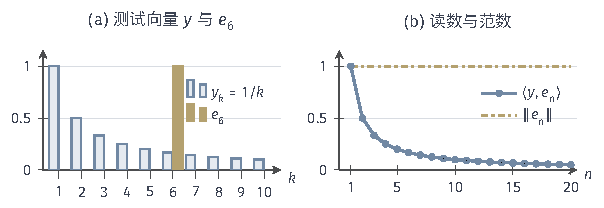
\includegraphics[width=102.3mm]{figures/02-abstract-mathematics/03-function-spaces/tikz/c2-weak-unit-vectors/figure.pdf}
  \caption{$\ell^2$中标准单位向量的弱收敛。(a)~固定读数$y_k=1/k$（浅蓝柱）与$e_6$（黄柱）只在第$6$个坐标重叠；(b)~读数$\langle y,e_n\rangle=1/n$（蓝）趋于零，而范数$\|e_n\|=1$（黄点划线）保持不变。每个固定读数都看到序列趋于零，整体误差却不减小。}
  \label{fig:lfo-weak-unit-vectors}
\end{figure}

\paragraph{振荡的函数}
函数空间中最典型的弱收敛来自振荡。在$L^2(0,2\pi)$中，$\sin(nx)/\sqrt\pi$是标准正交序列，所以$\sin(nx)\rightharpoonup0$。具体地取读数$g=\mathbf 1_{[0,1]}$，得$\int_0^1\sin(nx)\,dx=(1-\cos n)/n\to0$，而$\|\sin(nx)\|_2=\sqrt\pi$保持不变。函数在正负之间越来越快地摆动，任何固定的权重与它相乘再积分时，正负部分都相互抵消。

\paragraph{与测度弱收敛的区别}
第~\ref{sec:measure-sequence-convergence}节也有一个“弱收敛”，但对象和测试都不同。那里变化的是测度$\mu_n$，测试对象是有界连续函数，要求$\int f\,d\mu_n\to\int f\,d\mu$；这里变化的是一个固定线性空间中的元素，测试对象来自该空间的对偶。例如$\delta_{1/n}$作为测度弱收敛到$\delta_0$，但若把它们看成$C([0,1])^*$中的元素，它们之间的全变差距离始终为$2$，在对偶范数下并不收敛；两者的关系要通过第~\ref{sec:lfo-weak-star}节的弱星收敛来说明。两个定义同名，不能只凭名字互换。

\subsection{逐点有界与一致有界}
\label{sec:lfo-uniform-boundedness}

弱收敛只给出逐个读数的信息。我们自然要问：从“每个固定输入上都受控”能否推出某种统一的控制？本小节在Banach空间上给出肯定回答，下一小节再把它用于弱收敛列。

\paragraph{量词能否交换}
设$\{A_\alpha\}_{\alpha\in I}$是$\mathcal B(X,Y)$中的一族算子，并且对每个固定的$x$，$\sup_\alpha\|A_\alpha x\|<\infty$，称为逐点有界。问题是能否推出$\sup_\alpha\|A_\alpha\|<\infty$，即一致有界。前者是“对每个$x$，存在常数$C_x$”，后者是“存在常数$C$，对每个单位$x$”，两者的量词次序不同。

不完备的空间中，答案是否定的。在只有有限项非零的数列组成的空间$c_{00}$上配一致范数，令$L_n(x)=nx_n$。对固定的$x$，$n$超过最后一个非零坐标后$L_n(x)=0$，所以$\sup_n|L_n(x)|<\infty$；可是$\|L_n\|=n$，没有统一上界。下面会看到，完备性正是把逐点有界转为一致有界的关键。

\paragraph{Baire定理}
需要的工具是完备度量空间的一个性质：它不能写成可数个“很瘦”的闭集之并。这一性质称为\term{Baire纲定理}（Baire category theorem）。

\begin{theorem}[Baire纲定理]
\label{thm:lfo-baire}
设$(X,d)$是非空完备度量空间，$F_1,F_2,\ldots$是闭集且$X=\bigcup_kF_k$。则至少有一个$F_k$包含某个开球。
\end{theorem}

\begin{proof}
设每个$F_k$都不含开球，下面构造一个不属于任何$F_k$的点。$F_1$不含开球，所以$X\setminus F_1$是非空开集，可以取闭球$\overline B(x_1,r_1)\subset X\setminus F_1$，$r_1<1$。$F_2$不含开球，所以开球$B(x_1,r_1)$中有点不在$F_2$中，又因$F_2$闭，可取$\overline B(x_2,r_2)\subset B(x_1,r_1)\setminus F_2$，$r_2<1/2$。如此继续，得到嵌套闭球$\overline B(x_k,r_k)$，$r_k<1/k$，且第$k$个球与$F_k$不交。

球心满足$d(x_k,x_m)<r_k$（$m>k$），所以$(x_k)$是Cauchy列。由完备性，$x_k\to x$；每个闭球包含此后的全部球心，故$x\in\overline B(x_k,r_k)$对一切$k$成立，从而$x\notin F_k$对一切$k$成立，与$X=\bigcup_kF_k$矛盾。
\end{proof}

完备性在证明中只用了一次，即保证嵌套球心的极限存在。在$c_{00}$中，同样的嵌套构造可以逼近一个有无穷多非零项的数列，这个极限不在空间中，论证因此失效。下面的\term{一致有界原理}（uniform boundedness principle）把Baire定理用于算子族。

\begin{theorem}[一致有界原理]
\label{thm:lfo-uniform-boundedness}
设$X$是Banach空间，$Y$是赋范空间，$\{A_\alpha\}_{\alpha\in I}\subset\mathcal B(X,Y)$逐点有界，即对每个$x\in X$有$\sup_\alpha\|A_\alpha x\|<\infty$。则$\sup_\alpha\|A_\alpha\|<\infty$。
\end{theorem}

证明按“闭集覆盖—Baire定理给出内点—平移—缩放”的顺序展开。

\begin{proof}
\emph{第一步：层级闭集覆盖空间。}令$F_k=\{x\in X:\sup_\alpha\|A_\alpha x\|\leq k\}$。每个集合$\{x:\|A_\alpha x\|\leq k\}$由连续函数$x\mapsto\|A_\alpha x\|$定义，是闭集，$F_k$是它们的交，也是闭集。逐点有界说明每个$x$属于某个$F_k$，所以$X=\bigcup_kF_k$。

\emph{第二步：某一层含有开球。}$X$完备，由Baire定理，存在$k_0$和开球$B(x_0,r)\subset F_{k_0}$。

\emph{第三步：平移到原点。}对任意$\|z\|<r$，$x_0+z$与$x_0$都在$F_{k_0}$中，于是对每个$\alpha$，
\[
 \|A_\alpha z\|=\|A_\alpha(x_0+z)-A_\alpha x_0\|\leq k_0+k_0=2k_0 .
\]

\emph{第四步：缩放得到统一界。}对任意单位向量$x$及$0<s<r$，$\|sx\|<r$，由上一步$\|A_\alpha x\|=s^{-1}\|A_\alpha(sx)\|\leq2k_0/s$。令$s\to r$，得$\|A_\alpha\|\leq2k_0/r$对一切$\alpha$成立。
\end{proof}

图~\ref{fig:lfo-baire-layers}示意了这个论证。层级集$F_k=kF_1$是对称的闭凸集，一层套一层地覆盖整个空间；Baire定理保证某一层$F_{k_0}$中有一个小球。把这个球平移到原点，两点之差的估计使所有算子在原点附近的小球上一致受控，再用线性缩放推到整个单位球。

\begin{figure}[!htb]
  \centering
  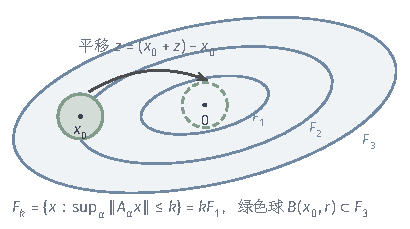
\includegraphics[width=69.3mm]{figures/02-abstract-mathematics/03-function-spaces/tikz/c2-baire-layers/figure.pdf}
  \caption{一致有界原理证明的示意。层级集$F_k=\{x:\sup_\alpha\|A_\alpha x\|\leq k\}$（蓝色嵌套区域）闭、对称且$F_k=kF_1$，它们的并是全空间。Baire定理给出某层（此处$F_3$）中的开球$B(x_0,r)$（绿）；平移到原点后，$z=(x_0+z)-x_0$使$\|z\|<r$时$\|A_\alpha z\|\leq2k_0$，缩放即得$\|A_\alpha\|\leq2k_0/r$。形状只是示意。}
  \label{fig:lfo-baire-layers}
\end{figure}

\paragraph{强收敛的算子列有统一界}
一致有界原理的第一个推论回答了第~\ref{sec:lfo-operator-convergence}节末尾的问题。

\begin{theorem}[Banach--Steinhaus]
\label{thm:lfo-banach-steinhaus}
设$X$是Banach空间，$Y$是赋范空间，$A_n\in\mathcal B(X,Y)$，并且对每个$x$，极限$Ax=\lim_nA_nx$存在。则$\sup_n\|A_n\|<\infty$，$A$是有界线性算子，且$\|A\|\leq\liminf_n\|A_n\|$。
\end{theorem}

\begin{proof}
收敛序列有界，所以$\{A_n\}$逐点有界，由定理~\ref{thm:lfo-uniform-boundedness}一致有界。$A$的线性由极限的线性得到。对单位向量$x$，$\|Ax\|=\lim_n\|A_nx\|\leq\liminf_n\|A_n\|$，对$x$取上确界即得。
\end{proof}

在截断投影的例子中，$\|P_n\|=1$，强极限$I$的范数也是$1$。这个推论说明，Banach空间上的强算子极限不会失去有界性，但它不能改进为算子范数收敛。

\paragraph{同一基础的后续用途}
完备性使量词交换成立，这个基础还会在第~\ref{sec:lfo-open-mapping}节的开映射定理中再用一次，届时直接调用Baire定理，不再重复建立。

\subsection{弱收敛列的范数控制}
\label{sec:lfo-weak-norm}

现在把一致有界原理用于弱收敛列。弱收敛只控制逐个读数，但我们将看到它仍然控制了两件事：序列的范数有统一上界，极限的范数不超过序列范数的下极限。

\begin{theorem}[弱收敛列有界且范数下半连续]
\label{thm:lfo-weak-bounded}
设$X$是赋范空间，$x_n\rightharpoonup x$。则$\sup_n\|x_n\|<\infty$，并且
\begin{equation}
 \|x\|\leq\liminf_{n\to\infty}\|x_n\| .
 \label{eq:lfo-weak-lsc}
\end{equation}
\end{theorem}

\begin{proof}
\emph{有界性。}把每个$x_n$看成对偶空间上的读数：$J_n(L)=L(x_n)$，$L\in X^*$。$J_n$是$X^*$上的线性泛函，它的范数是单位读数在$x_n$上的最大读值，由定理~\ref{thm:lfo-norming-functional}恰好等于$\|x_n\|$。对每个固定的$L$，$J_n(L)=L(x_n)$收敛，因而有界，所以$\{J_n\}$在$X^*$上逐点有界。$X^*$总是Banach空间，由定理~\ref{thm:lfo-uniform-boundedness}得$\sup_n\|x_n\|=\sup_n\|J_n\|<\infty$。

\emph{下半连续。}任取$\|L\|\leq1$，则$|L(x)|=\lim_n|L(x_n)|\leq\liminf_n\|x_n\|$。对$L$取上确界，由式~\eqref{eq:lfo-norm-dual}得式~\eqref{eq:lfo-weak-lsc}。
\end{proof}

证明中用到的完备空间是$X^*$而不是$X$，所以这个结论对不完备的$X$也成立。

\paragraph{不弱收敛的放大序列}
定理给出了一个检验：无界的序列不可能弱收敛。在$\ell^2$中，$\sqrt n\,e_n$的范数趋于无穷，所以它不弱收敛。可以直接找到证据：取$y_k=k^{-3/4}$，$\sum_kk^{-3/2}<\infty$，$y\in\ell^2$，而$\langle y,\sqrt n\,e_n\rangle=n^{1/4}\to\infty$。

\paragraph{范数可以在极限中下降}
式~\eqref{eq:lfo-weak-lsc}可以是严格不等式：$e_n\rightharpoonup0$，$\|0\|=0<1=\liminf\|e_n\|$。弱收敛允许一部分“能量”在极限中消失，例如振荡的$\sin(nx)$弱收敛到零而范数保持$\sqrt\pi$。

\paragraph{Hilbert空间：弱收敛加范数收敛得强收敛}
如果范数没有下降，在Hilbert空间中就能恢复强收敛。设$x_n\rightharpoonup x$且$\|x_n\|\to\|x\|$，展开
\[
 \|x_n-x\|^2=\|x_n\|^2-2\operatorname{Re}\langle x,x_n\rangle+\|x\|^2\longrightarrow\|x\|^2-2\|x\|^2+\|x\|^2=0 .
\]
这里用到了弱收敛$\langle x,x_n\rangle\to\langle x,x\rangle$和内积恒等式。这一步依靠内积，不能作为任意Banach空间的结论。

\paragraph{一般Banach空间中的反例}
在$C([0,1])$中，令$h(t)=\max(0,2t-1)$，$g_n$为支撑在$[0,2/n]$上、在$t=1/n$处取峰值$1$的三角尖峰，$f_n=h+g_n$。$n\geq4$时两部分支撑不交，$\|f_n\|_\infty=1=\|h\|_\infty$。由定理~\ref{thm:lfo-ck-dual}，每个读数都是对某个有限符号测度$\mu$积分；$g_n$一致有界且逐点趋于零，由控制收敛定理$\int g_n\,d\mu\to0$，所以$f_n\rightharpoonup h$。然而$\|f_n-h\|_\infty=\|g_n\|_\infty=1$，不收敛。图~\ref{fig:lfo-weak-norm-drop}画出了这个序列：尖峰贴着左端点越来越窄，不改变最大值，也躲开了每一个固定的测度。

\begin{figure}[!htb]
  \centering
  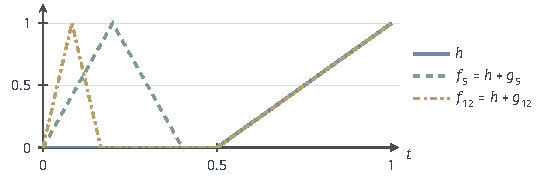
\includegraphics[width=92.8mm]{figures/02-abstract-mathematics/03-function-spaces/tikz/c2-weak-norm-drop/figure.pdf}
  \caption{一致范数下弱收敛加范数收敛不推出强收敛。$h(t)=\max(0,2t-1)$（蓝），$f_n=h+g_n$，其中$g_n$是支撑在$[0,2/n]$、峰值为$1$的尖峰；图中为$n=5$（绿虚线）与$n=12$（黄点划线）。$\|f_n\|_\infty=\|h\|_\infty=1$，$f_n\rightharpoonup h$，但$\|f_n-h\|_\infty=1$。}
  \label{fig:lfo-weak-norm-drop}
\end{figure}

\subsection{Hilbert空间中的弱收敛子列}
\label{sec:lfo-weak-subsequence}

有限维中，有界序列总有收敛子列；无限维中$e_n$说明这对范数收敛不成立。弱收敛的要求更低，本小节证明在Hilbert空间中它恢复了这个性质。

\begin{theorem}[Hilbert空间中的弱子列]
\label{thm:lfo-weak-subsequence}
Hilbert空间中的每个有界序列都有弱收敛的子列。
\end{theorem}

先在可分情形用标准正交基把问题化为系数列，再推广到一般情形。

\begin{proof}
设$\|x_n\|\leq C$。

\emph{第一步：逐个系数抽子列。}先设$H$可分，取标准正交基$(e_k)$，记系数$c_{n,k}=\langle e_k,x_n\rangle$，$|c_{n,k}|\leq C$。有界数列有收敛子列：先从$(x_n)$中抽子列使第$1$个系数收敛，再从中抽子列使第$2$个系数收敛，如此继续。取第$j$个子列的第$j$项组成对角子列$(x_{n_j})$，它从某项起是每个子列的子列，所以对每个$k$，$c_{n_j,k}\to a_k$。

\emph{第二步：极限系数平方可和。}对任意有限的$K$，$\sum_{k\leq K}|a_k|^2=\lim_j\sum_{k\leq K}|c_{n_j,k}|^2\leq C^2$，后一个不等式是Bessel不等式。令$K\to\infty$，$\sum_k|a_k|^2\leq C^2$，所以$x=\sum_ka_ke_k\in H$，$\|x\|\leq C$。

\emph{第三步：对所有方向收敛。}任取$y\in H$及$\varepsilon>0$，取$K$使$\|y-P_Ky\|<\varepsilon$，其中$P_K$是到前$K$个基向量的投影。分解
\[
 \langle y,x_{n_j}-x\rangle=\langle P_Ky,x_{n_j}-x\rangle+\langle y-P_Ky,x_{n_j}-x\rangle .
\]
第一项是有限个系数之差的线性组合，随$j\to\infty$趋于零；第二项不超过$\varepsilon\cdot2C$。所以$\limsup_j|\langle y,x_{n_j}-x\rangle|\leq2C\varepsilon$，由$\varepsilon$任意得$x_{n_j}\rightharpoonup x$。

\emph{第四步：一般Hilbert空间。}令$M$为$\{x_n\}$的闭线性张成。有理系数（复情形为实部虚部都有理）的有限线性组合在$M$中稠密，所以$M$可分，对$M$应用前三步得到子列与$x\in M$，使对一切$y\in M$弱收敛成立。对一般的$y\in H$，写$y=P_My+(y-P_My)$，后者与$M$正交，从而与每个$x_n$及$x$的内积都是零，故$\langle y,x_{n_j}\rangle=\langle P_My,x_{n_j}\rangle\to\langle P_My,x\rangle=\langle y,x\rangle$。
\end{proof}

\paragraph{坐标收敛还不够}
第三步不能省略：逐个系数收敛本身并不等于弱收敛。$x_n=n\,e_n$的每个坐标都最终为零，坐标逐点收敛到零向量，但取$y_k=1/k$，$\langle y,x_n\rangle=1$不趋于零。证明中让有限截断与尾项估计配合的，是序列的统一界$C$；有界性加坐标收敛才推出弱收敛。

\paragraph{弱子列不是范数紧性}
定理只保证弱收敛的子列。单位向量$e_n$本身就弱收敛到零，但没有范数收敛的子列，所以单位球在范数下不紧。弱极限也不必保留序列满足的约束：每个$e_n$都在单位球面$\{\|x\|=1\}$上，弱极限$0$却不在。哪些约束集在弱极限下封闭（例如闭凸集），以及由此得到的极小值存在性，属于优化问题中的存在性讨论，与第~\ref{sec:lfo-finite-observations}节末提到的拟合问题一样留给卷三的优化部分。

\subsection{反射空间的弱紧性（补充）}
\label{sec:lfo-reflexive}

上一小节的证明利用了标准正交基。离开Hilbert空间，有界序列是否仍有弱收敛子列？答案取决于空间与它的二次对偶的关系。

\paragraph{自然嵌入与反射}
每个$x\in X$都给出对偶空间上的一个读数：$(Jx)(L)=L(x)$，$L\in X^*$。$J:X\to X^{**}$线性，由定理~\ref{thm:lfo-norming-functional}，$\|Jx\|=\sup_{\|L\|\leq1}|L(x)|=\|x\|$，所以$J$是保范数的嵌入，称为\term{自然嵌入}（canonical embedding）。若$J$是满射，即$X^{**}$的每个元素都是某个$x$对应的读数，则称$X$为\term{反射空间}（reflexive space）。反射空间必然完备，因为$X^{**}$作为对偶空间是完备的。

有限维空间和Hilbert空间都是反射的：后者用两次Riesz表示即可验证。对$1<p<\infty$，由定理~\ref{thm:lfo-lp-dual}，$(L^p)^*\cong L^q$，$(L^q)^*\cong L^p$，逐层追踪对应关系可以验证合成后正是$J$，所以$L^p$是反射的。第~\ref{sec:lfo-lp-dual}节的端点讨论则表明$\ell^1$不是反射的：它的二次对偶是$(\ell^\infty)^*$，严格大于$\ell^1$。

\begin{theorem}[反射空间的弱紧性]
\label{thm:lfo-reflexive-compact}
设$X$是反射Banach空间。则$X$的闭单位球在弱拓扑下紧，并且$X$中每个有界序列都有弱收敛的子列。
\end{theorem}

\paragraph{为什么要单独陈述序列结论}
弱拓扑一般不能由度量给出，所以第~\ref{sec:metric-compact-sequential-tests}节中“紧等价于序列紧”的结论不能直接套用；从紧性推出序列结论需要另一个定理（Eberlein--Šmulian定理）。对序列结论，可以给一个直接的证明思路：令$Y$为序列的闭线性张成，它可分且反射；由$Y^{**}=J(Y)$可分可推出$Y^*$可分；在$Y^*$的可数稠密集上逐个对角化，得到使每个读数$L(x_{n_j})$都收敛的子列；极限读数是$Y^{**}$的元素，由反射性对应某个$x\in Y$；最后用Hahn--Banach定理把$X^*$中的读数限制到$Y$上，得到$x_{n_j}\rightharpoonup x$。一般证明属于补充。

\paragraph{$L^1$中质量集中的序列}
有界性在非反射空间中不足以保证弱子列。在$L^1(0,1)$中令$f_n=n\mathbf 1_{(0,1/n)}$，$\|f_n\|_1=1$。设某个子列$f_{n_j}\rightharpoonup f\in L^1$。对任意$0<a<1$，取读数$g=\mathbf 1_{(a,1)}\in L^\infty$；当$n_j>1/a$时$\int_a^1f_{n_j}\,dt=0$，所以$\int_a^1f\,dt=0$。对一切$a$成立，相减得$f$在每个区间$(a,b)\subset(0,1)$上积分为零，从而$f=0$几乎处处。但取读数$g\equiv1$，$\int_0^1f_{n_j}\,dt=1$，又得$\int_0^1f\,dt=1$，矛盾。

图~\ref{fig:lfo-escaping-mass}画出了这一列：质量始终为$1$，却向左端点越挤越窄。远离零点的读数（灰色区域）看到的是零，整体积分看到的却是一。极限对象应当是Dirac测度$\delta_0$，它不是$L^1$中的函数，这一列在$L^1$中找不到弱极限。所以第~\ref{sec:lfo-weak-subsequence}节和本小节的结论不能无条件推广到$L^1$或$L^\infty$。

\begin{figure}[!htb]
  \centering
  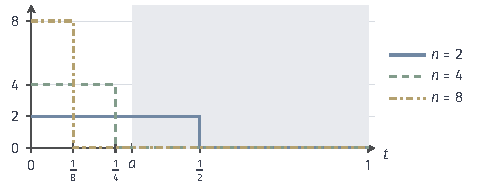
\includegraphics[width=80.8mm]{figures/02-abstract-mathematics/03-function-spaces/tikz/c2-escaping-mass/figure.pdf}
  \caption{$L^1(0,1)$中有界但没有弱收敛子列的序列$f_n=n\mathbf 1_{(0,1/n)}$，图中$n=2,4,8$。每个$f_n$的积分都为$1$；灰色区域是读数$\mathbf 1_{(a,1)}$（$a=0.3$）的支撑，$n>1/a$后在该区域上的积分为零。远离原点的读数迫使候选极限几乎处处为零，整体积分却保持为$1$，二者不能同时满足。}
  \label{fig:lfo-escaping-mass}
\end{figure}

\subsection{对偶空间的弱星紧性（补充）}
\label{sec:lfo-weak-star}

上面的$f_n\,dt$若看成$C([0,1])$上的读数，确实“收敛”到$\delta_0$：对每个连续$u$，$\int_0^1uf_n\,dt\to u(0)$。这提示我们，当变化的对象本身是读数时，可以只用原空间的元素去测试它们。

\begin{definition}[弱星收敛]
\label{def:lfo-weak-star}
设$X$是赋范空间，$L_n,L\in X^*$。若对每个$x\in X$都有$L_n(x)\to L(x)$，则称$L_n$\term{弱星收敛}（weak-star convergence）到$L$，记为$L_n\overset{*}{\rightharpoonup}L$。
\end{definition}

$X^*$本身是Banach空间，它也有自己的弱收敛，测试对象是$X^{**}$的全部元素；弱星收敛只用自然嵌入的像$J(X)\subset X^{**}$测试，要求更少。所以在$X^*$中，弱收敛蕴含弱星收敛，$X$反射时二者一致。

\paragraph{Banach--Alaoglu定理}
弱星收敛的好处是紧性在任何对偶空间中都成立，不需要反射性，这就是\term{Banach--Alaoglu定理}（Banach--Alaoglu theorem）。

\begin{theorem}[Banach--Alaoglu]
\label{thm:lfo-banach-alaoglu}
设$X$是赋范空间。则$X^*$的闭单位球在弱星拓扑下紧。
\end{theorem}

这里的紧性所对应的测试对象是原空间$X$。一般证明把单位球嵌入乘积空间$\prod_{x\in X}[-\|x\|,\|x\|]$，再用Tychonoff定理，属于补充。和反射空间一样，一般的弱星紧性不直接给出序列结论；下面在前对偶$X$可分的条件下给出直接证明。

\begin{theorem}[可分前对偶下的弱星子列]
\label{thm:lfo-weak-star-sequential}
设$X$是可分赋范空间。则$X^*$中每个有界序列都有弱星收敛的子列。
\end{theorem}

\begin{proof}
设$\|L_n\|\leq C$，$\{z_k\}$是$X$的可数稠密子集。对每个$k$，$(L_n(z_k))_n$是有界数列；与定理~\ref{thm:lfo-weak-subsequence}的第一步相同，逐个$k$抽子列再取对角，得到子列$(L_{n_j})$，使$L_{n_j}(z_k)$对每个$k$都收敛。

对一般的$x\in X$及$\varepsilon>0$，取$z_k$使$\|x-z_k\|<\varepsilon$，则
\[
 \begin{aligned}
 |L_{n_i}(x)-L_{n_j}(x)|
 &\leq|L_{n_i}(x-z_k)|+|L_{n_i}(z_k)-L_{n_j}(z_k)|+|L_{n_j}(z_k-x)|\\
 &\leq2C\varepsilon+|L_{n_i}(z_k)-L_{n_j}(z_k)| .
 \end{aligned}
\]
最后一项在$i,j$充分大时小于$\varepsilon$，所以$(L_{n_j}(x))$是Cauchy数列，极限记为$L(x)$。$L$是线性的，且$|L(x)|\leq C\|x\|$，故$L\in X^*$，$L_{n_j}\overset{*}{\rightharpoonup}L$。
\end{proof}

统一的范数界$C$在证明中起了关键作用：它把可数个测试点上的收敛推广到所有测试点。可分性则保证只需对可数个测试点对角化。

\paragraph{$L^\infty$中的振荡}
$L^\infty(0,1)$是可分空间$L^1(0,1)$的对偶，所以其中的有界序列有弱星收敛的子列。取$g_n(t)=\operatorname{sgn}(\sin(2\pi nt))$，它在$2n$个等长小区间上交替取$\pm1$，$\|g_n\|_\infty=1$。对区间的示性函数$f=\mathbf 1_{(a,b)}$，$\int g_nf\,dt$只来自两端不完整的小区间，绝对值不超过$1/n$，趋于零；由线性对阶梯函数成立，再由阶梯函数在$L^1$中稠密及统一界$\|g_n\|_\infty=1$推广到一切$f\in L^1$。所以$g_n\overset{*}{\rightharpoonup}0$，而$\|g_n-g_m\|_\infty$不趋于零，序列不按范数收敛。

同样，$C([0,1])$可分，本小节开头的$f_n\,dt$作为$C([0,1])^*$中的有界序列弱星收敛到$\delta_0$。在$L^1$中找不到的极限，在更大的对偶空间$C([0,1])^*$中以测度的形式出现了。

\paragraph{可分性不能省}
若前对偶不可分，序列结论可以失效。$\ell^\infty$不可分；考虑其对偶中的读数$L_n(x)=x_n$，$\|L_n\|=1$。对任意子列$(L_{n_j})$，取$x\in\ell^\infty$使$x_{n_j}=(-1)^j$（其余坐标为零），则$L_{n_j}(x)=(-1)^j$不收敛。所以这个有界序列没有弱星收敛的子列，尽管Banach--Alaoglu定理仍保证单位球弱星紧。可分性必须写在序列结论之前。
